\documentclass[conference]{IEEEtran}
\IEEEoverridecommandlockouts
\usepackage{cite}
\usepackage{amsmath,amssymb,amsfonts}
\usepackage{graphicx}
\usepackage{booktabs}
\usepackage{textcomp}
\usepackage{xcolor}
\usepackage{url}
\usepackage[utf8]{inputenc}
\usepackage{newunicodechar}
\newunicodechar{×}{\ensuremath{\times}}
\newunicodechar{≈}{\ensuremath{\approx}}
\newunicodechar{σ}{\ensuremath{\sigma}}
\newunicodechar{–}{--}
\newunicodechar{—}{---}
\newunicodechar{±}{\ensuremath{\pm}}
\newunicodechar{→}{\ensuremath{\rightarrow}}
\newunicodechar{≥}{\ensuremath{\geq}}
\newunicodechar{Δ}{\ensuremath{\Delta}}
\newunicodechar{†}{\ensuremath{\dagger}}
\newunicodechar{“}{``}
\newunicodechar{”}{''}
\newunicodechar{’}{'}
\newunicodechar{≤}{\ensuremath{\leq}}
\newunicodechar{✓}{\ensuremath{\checkmark}}
\begin{document}
\title{Localize to Detect: Full-Resolution Deep Forensics and Compression Cues for GPT-Image-2 Field Forgeries in Receipts and Forms}
\author{
\IEEEauthorblockN{Omkar Suryavanshi}\IEEEauthorblockA{\textit{B.Tech CSE (AIML)} \\ \textit{D. Y. Patil International University}\\ Akurdi, Pune, India \\ 20240802073@dypiu.ac.in}}
\maketitle
\begin{abstract}
Instruction-following image generators can rewrite a single price, date or phone number inside a scanned receipt so convincingly that human inspectors and off-the-shelf forensic detectors perform near chance. We study this threat on AIForge-Doc v2, a paired benchmark of 3,066 GPT-Image-2 field forgeries with pixel-aligned authentic originals and tampering masks. We remove 31 duplicated source documents (6 of which leak across the official train/test split) and score both versions of every test document. Because the forged field covers a median of only 0.76\% of the page, page-level recipes fail: raw-pixel logistic regression scores AUC 0.504 and a fine-tuned ResNet-50 on resized pages 0.501. We propose FieldForensics, a \emph{localize-to-detect} U-Net that fuses RGB with an SRM noise residual at native resolution, is trained on field-centred crops with \emph{paired hard negatives}, and scores a page by the peak of its tampering map. On 1,212 held-out images it reaches an AUC of 0.933 (95\% CI [0.919, 0.945]), a paired two-alternative forced-choice accuracy of 92.9\% and a pixel F1 of 0.667, against published zero-shot AUCs of 0.585--0.599 for DocTamper and TruFor and 0.501 for humans. Block-wise compression statistics (ELA, noise, blockiness) are a strong baseline (AUC 0.817) because they exploit the compression-history mismatch of the pasted field. The clean-trained network learns this cue by itself, whereas a variant trained with degradation augmentation (FieldForensics-R, 0.839) suppresses it and recovers it only through fusion with the statistics (0.893). Under JPEG-75 re-compression the statistics fall to chance (0.513), FieldForensics to 0.608 and FieldForensics-R to 0.675, which exposes a trade-off between clean accuracy and robustness.
\end{abstract}
\begin{IEEEkeywords}
Document forensics, AI-generated image detection, generative inpainting, tampered text localization, GPT-Image-2, AIForge-Doc, noise residual, robustness
\end{IEEEkeywords}
\section{Introduction}\label{sec:intro}
Receipts, invoices, bank statements and filled-in forms are routinely accepted as evidence in expense reimbursement, insurance claims, loan applications and know-your-customer checks. Traditional document fraud---copy--move of digits, splicing of text from another document, or font substitution in an editor---leaves traces that forensic detectors have learned to exploit, such as double-JPEG compression, resampling and inconsistent noise \cite{findit,doctamper,catnet}. Instruction-following image generators have changed this picture. A forger can now mark a field and ask a model to ``replace 1,346,000 with 2,103,717 in the same font'', and the generator synthesises the new glyphs with matching ink texture, paper colour, blur and perspective. Fig.~\ref{fig:teaser} shows such a forgery and how our detector exposes it.

\begin{figure*}[t]
\centering
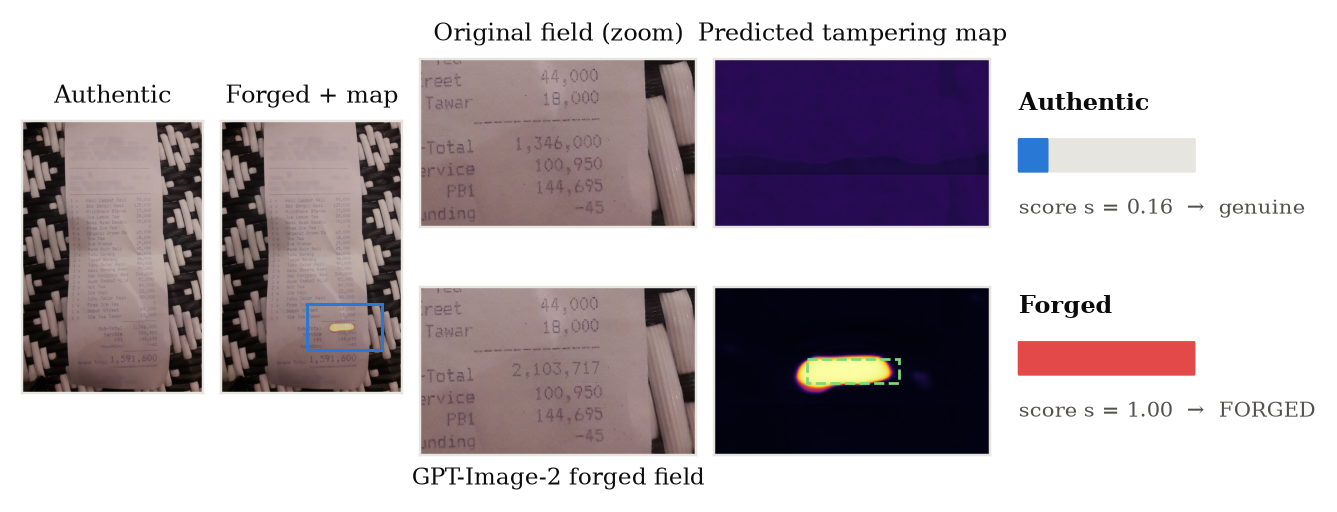
\includegraphics[width=\textwidth]{figures/teaser.png}
\caption{FieldForensics at a glance. A GPT-Image-2 forgery changes a single subtotal (1,346,000 $\rightarrow$ 2,103,717) on a CORD receipt, invisible at page scale. Our network analyses the page at native resolution and outputs a tampering map that lights up exactly on the regenerated digits (dashed: ground-truth field). The page score is the peak of the map: 1.00 for the forgery and 0.16 for the untouched original.}
\label{fig:teaser}
\end{figure*}
AIForge-Doc \cite{aiforge1} and its second version \cite{aiforge2} quantify how serious this is. In v2, 3,066 numeric or key fields from four public receipt and form corpora \cite{cord,wildreceipt,sroie,xfund} were rewritten by OpenAI's GPT-Image-2 and pasted back into the original page. The benchmark authors report that human inspectors in a two-alternative forced-choice study achieve an AUC of 0.501, the state-of-the-art general forensic detector TruFor \cite{trufor} 0.599, the document-specific detector DocTamper \cite{doctamper} 0.585, and GPT-Image-2 judging its own forgeries 0.532 \cite{aiforge2,forgerjudge}. Both detectors exceed 0.85 AUC on traditional tampering of the same source documents, which isolates an \emph{AI-inpainting-specific} detection gap.

The present work began as a course project whose first report trained a logistic regression on down-sampled document images and compared centre, random and text-density crops. In hindsight that design could not succeed: the forged field occupies a median of 0.76\% of the page (5th--95th percentile: 0.03--2.8\%), so resizing a 2480$\times$3508 form to a thumbnail erases the evidence, and fixed crops usually miss the field altogether. This paper replaces that study with a rigorous re-design built on one principle: \emph{to decide whether a document has been forged, first find where it could have been forged, at the resolution at which the forgery was made}.

Our contributions are as follows:

\begin{itemize}
\item \textbf{A leak-free, paired evaluation protocol for AIForge-Doc v2.} We verify that every forged image is pixel-identical to its authentic counterpart outside the mask, remove 31 duplicated source documents (6 of which straddle the official train/test split), and score both versions of each of the 606 remaining test documents, so that classifiers cannot exploit document identity, layout or source.
\item \textbf{FieldForensics, a localize-to-detect architecture.} A U-Net \cite{unet} with a ResNet-34 \cite{resnet} encoder fuses RGB with a fixed SRM noise residual \cite{srm,rgbn}, keeps a full-resolution skip path for stroke-level detail, and is trained jointly for pixel localisation and image-level detection using field-centred crops with paired hard negatives.
\item \textbf{A broad empirical study} comparing classical and deep baselines, ablating the main design choices with paired bootstrap significance tests, and measuring per-source behaviour, sensitivity to forged-region size, robustness to realistic degradations and generalisation to unseen document sources.
\item \textbf{An analysis of the cues.} Block-wise compression statistics are a surprisingly strong baseline that exploits compression-history inconsistencies. A network trained on clean data learns these cues by itself, whereas degradation augmentation suppresses them. The result is a clear trade-off between clean accuracy and robustness to re-compression, which we quantify, together with a document-type effect that masquerades as a forged-area effect.
\end{itemize}
\section{Related Work}\label{sec:rel}
\subsection{Document tampering detection}
Early document-forensics work relied on hand-crafted cues such as character alignment, font consistency and printer signatures; the ICPR 2018 \emph{Find it!} contest \cite{findit} established receipts as a benchmark domain. Deep approaches followed general image-manipulation detection: RGB-N \cite{rgbn} paired an RGB stream with an SRM noise stream \cite{srm}, ManTra-Net \cite{mantra} learned anomalous local features, MVSS-Net \cite{mvss} combined edge and noise supervision, CAT-Net \cite{catnet} exploited JPEG DCT statistics, and TruFor \cite{trufor} learned a camera-noise fingerprint (Noiseprint++) with a reliability map. DocTamper \cite{doctamper} adapted these ideas to text images using frequency-domain features and multi-JPEG training. These detectors were designed for splicing, copy--move and classical inpainting, and AIForge-Doc shows that they transfer poorly to generative edits \cite{aiforge1,aiforge2}.

\subsection{AI-generated image detection}
Fully synthetic images can often be detected from generator fingerprints in the frequency spectrum \cite{wang2020,corvi} or from the feature space of large pretrained encoders \cite{ojha}, although generalisation to unseen generators and post-processing remains open \cite{li2025}. Deep inpainting of natural images has been localised with high-pass fully convolutional networks \cite{hpfcn}. Fu \emph{et al.} \cite{fu2026} showed that detectors trained on natural images do not carry over to documents, whose statistics are dominated by text, flat backgrounds and scanning artefacts. Field-level forgeries are the hardest case: the edited region is tiny and the remaining $>$99\% of pixels are genuine, so image-level fingerprints are diluted by authentic content.

\subsection{Benchmarks for AI-forged documents}
AIForge-Doc v1 \cite{aiforge1} introduced 4,062 forgery specifications executed with Gemini 2.5 Flash Image and Ideogram v2; v2 \cite{aiforge2} re-executes the same specifications with GPT-Image-2 and, crucially, releases the authentic source of every forgery, pixel-aligned, together with the tampering mask. Its authors evaluate detectors zero-shot; to the best of our knowledge we report the first supervised detectors and localisers trained and evaluated on the v2 split under a leak-free protocol.

\section{Dataset and Evaluation Protocol}\label{sec:data}
\subsection{AIForge-Doc v2}
Each forgery is produced in four steps \cite{aiforge2}: a numeric or key field (price, total, date, telephone number, document ID or form answer) is selected from the source annotation and a plausible replacement string is generated; the field box is enlarged by 50\% to give the generator context; GPT-Image-2 inpaints the box under a prompt that fixes the target string and asks for typography matching; and only the exact field box is pasted back into the full-resolution page, which is saved as a metadata-free PNG. Fig.~\ref{fig:examples} shows one example per source. Table~\ref{tab:data} summarises the composition after our de-duplication.

\begin{figure*}[t]
\centering
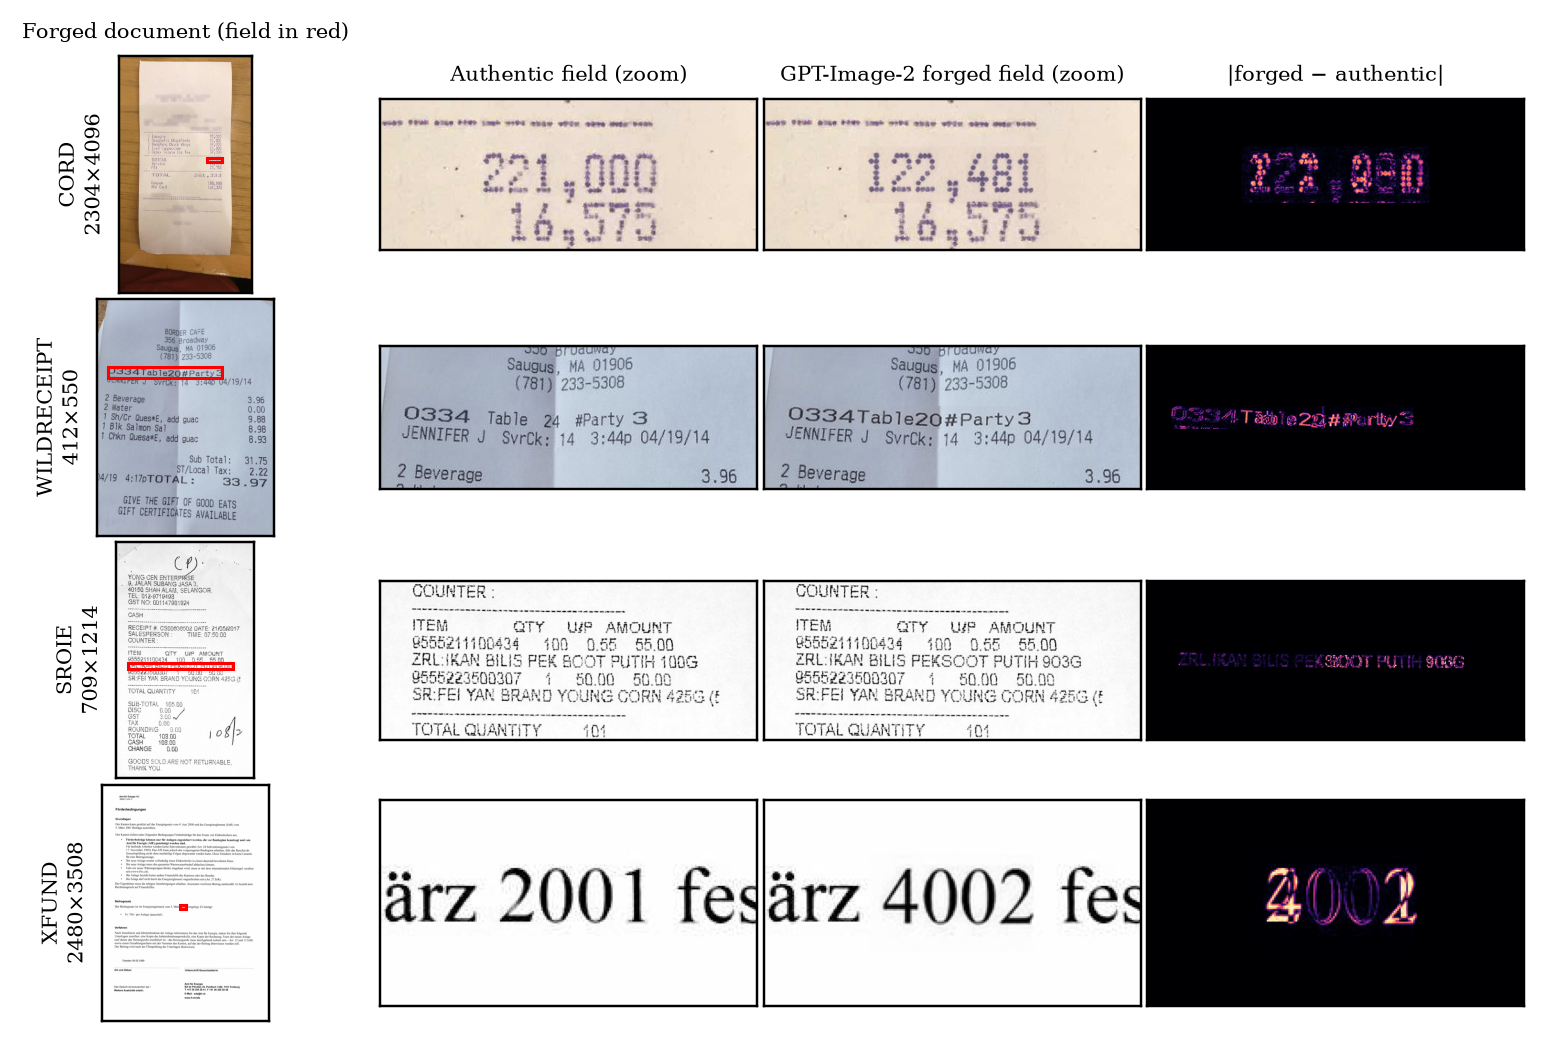
\includegraphics[width=\textwidth]{figures/examples.png}
\caption{One forged document per source. Left: full page with the forged field outlined. Middle: authentic and GPT-Image-2 versions of the field at native resolution. Right: absolute difference, which is non-zero only inside the field. The edits are visually seamless, and the forged area is a tiny fraction of the page.}
\label{fig:examples}
\end{figure*}
\begin{table}[t]
\centering
\caption{Composition of the de-duplicated AIForge-Doc v2 splits (documents; each contributes one authentic and one forged image)}
\label{tab:data}
\footnotesize
\setlength{\tabcolsep}{3pt}
\begin{tabular}{lccccc}
\toprule
Source & Type / orig. format & Train & Val & Test & Median size (px) \\
\midrule
CORD v2 \cite{cord} & receipt / PNG & 707 & 78 & 196 & 864$\times$1296 \\
WildReceipt \cite{wildreceipt} & receipt / JPEG & 962 & 107 & 267 & 348$\times$450 \\
SROIE \cite{sroie} & receipt / JPEG & 216 & 24 & 60 & 623$\times$1471 \\
XFUND \cite{xfund} & form / PNG & 301 & 34 & 83 & 2480$\times$3508 \\
Total &  & 2,186 & 243 & 606 &  \\
\bottomrule
\end{tabular}
\end{table}
Fig.~\ref{fig:stats} visualises three properties that drive our design. WildReceipt and CORD dominate the data (a). The forged region is tiny: its area spans three orders of magnitude, with XFUND fields covering only about 0.01--0.1\% of a page (b). Prices, totals and phone numbers, i.e. the fields a fraudster would actually target, make up most edits (c).

\begin{figure*}[t]
\centering
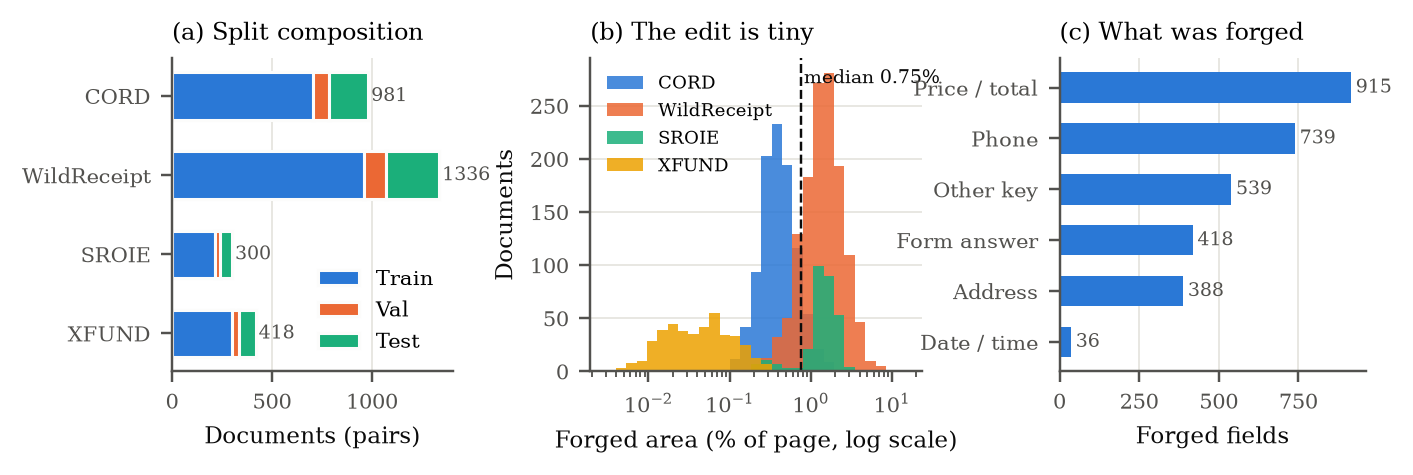
\includegraphics[width=\textwidth]{figures/dataset_stats.png}
\caption{AIForge-Doc v2 after de-duplication. (a) Documents per source and split. (b) Distribution of the forged area as a percentage of the page (log scale), by source; the dashed line marks the median of 0.76\%. (c) Types of forged fields.}
\label{fig:stats}
\end{figure*}
\subsection{Integrity audit and de-duplication}
Before any modelling we verified three properties programmatically. (i) For all 3,066 pairs the forged and authentic images are bit-identical outside the tampering mask, and each mask is exactly the axis-aligned field rectangle. (ii) The authentic SHA-256 hashes reveal 25 groups of byte-identical source images, i.e. the same receipt occurring under two different source identifiers. Six of these groups cross the official train/test boundary, which would let a model memorise a test document during training. We therefore drop the test copy of every cross-split duplicate and keep only one copy of within-split duplicates, removing 31 documents in total. (iii) From the remaining training documents we hold out a source-stratified 10\% validation set. The final split has 2,186 training, 243 validation and 606 test documents (Table~\ref{tab:data}).

\subsection{Paired protocol and metrics}
Every test document contributes both its authentic and its forged image (1,212 test images, perfectly balanced). Because the two images of a pair share source, size, layout, language and content except for one field, any score difference must come from the forged region itself. We report the area under the ROC curve (AUC) with 95\% confidence intervals from 2,000 bootstrap resamples of \emph{documents} (pairs are resampled together) \cite{bootstrap}; accuracy, precision, recall and F1 at the fixed decision threshold 0.5; the true-positive rate at 5\% false-positive rate (TPR@5\%FPR), an operating point relevant to fraud screening; and the \emph{paired accuracy}, the fraction of documents whose forged version receives a higher score than its authentic version. Paired accuracy is the two-alternative forced-choice (2AFC) metric used for the human study in \cite{aiforge2}. For localisation we report pixel F1 and IoU of the thresholded map on forged images, and the \emph{peak-hit rate}: how often the most suspicious location in the page lies inside the forged field. Differences between systems are tested with a paired bootstrap over documents.

\section{Method: FieldForensics}\label{sec:method}
\begin{figure*}[t]
\centering
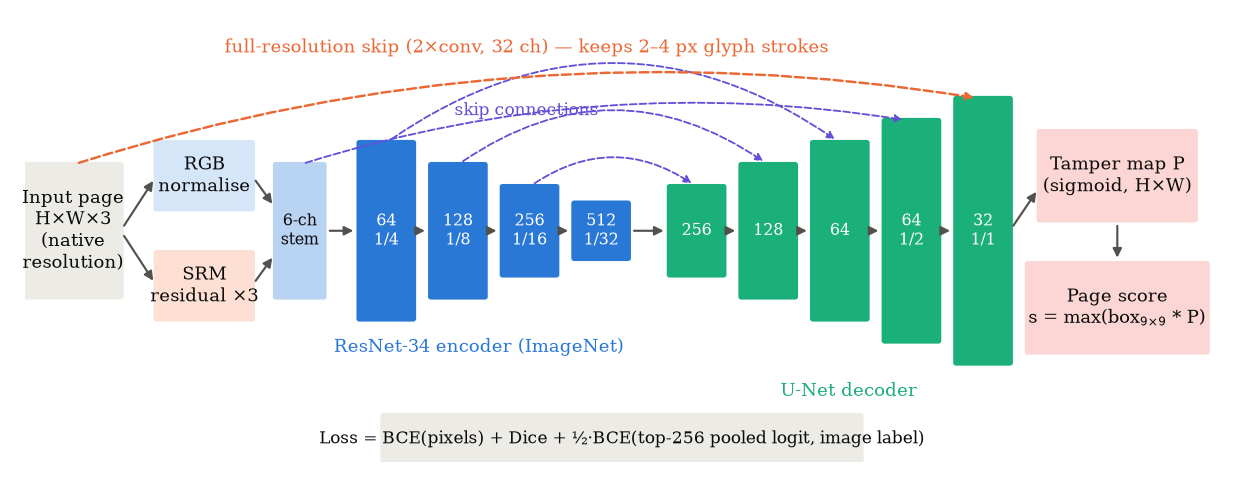
\includegraphics[width=\textwidth]{figures/method.png}
\caption{Overview of FieldForensics. The document is processed at native resolution. RGB and a fixed SRM noise residual are fused at the stem of a ResNet-34 U-Net with an additional full-resolution skip path. The network predicts a tampering-probability map, and the document score is the maximum of the smoothed map. Training uses field-centred crops with paired authentic negatives and a joint pixel/image loss.}
\label{fig:method}
\end{figure*}
\subsection{Problem formulation}
Given a document image $I \in \{0,\ldots,255\}^{H\times W\times 3}$, the goal is to output an image-level score $s(I)\in[0,1]$ that is high if any region was regenerated, together with a map $P\in[0,1]^{H\times W}$ that localises the regenerated pixels. Training provides, for each document, the authentic image $I^{a}$, the forged image $I^{f}$ and the field mask $M$. Since the forgery is local, we cast detection as localisation followed by pooling, in the spirit of multiple-instance learning \cite{mil}: a document is forged if and only if at least one location is forged.

\subsection{Architecture}
\emph{Input streams.} Generative inpainting reproduces the look of the glyphs well but not the sensor, print and compression noise of the surrounding scan \cite{hpfcn}. Besides the ImageNet-normalised RGB channels we therefore compute three fixed SRM high-pass residuals \cite{srm,rgbn} of the luminance $Y$: a second-order 3$\times$3 kernel $K_1$, the 5$\times$5 ``KV'' kernel $K_2$ and a horizontal second-order kernel $K_3$, truncated and normalised as

\begin{equation}
N_i = \frac{1}{3}\,\mathrm{clip}\left(K_i * Y,\,-3,\,3\right),\qquad i=1,2,3.
\label{eq:srm}
\end{equation}
RGB and noise are concatenated into a 6-channel input. The first convolution of an ImageNet-pretrained \cite{imagenet} ResNet-34 \cite{resnet} is extended to six channels: the RGB filters are copied and the noise filters are initialised with half the channel-mean of the RGB filters.

\emph{Decoder.} A U-Net decoder \cite{unet} upsamples the encoder features (strides 32 down to 2) through four skip connections. Because typical forged glyph strokes are only 2--4 pixels wide, we add a fifth, \emph{full-resolution} skip branch (two 3$\times$3 convolutions with 32 channels on the raw 6-channel input), so that the final prediction can use stroke-level evidence instead of interpolating from stride 2. A 1$\times$1 convolution produces the logit map $Z$, and $P=\sigma(Z)$. The network has 24.5\,M parameters and is fully convolutional, so it runs on pages of any size without resizing.

\subsection{Field-centred sampling with paired hard negatives}
Training uses $384\times384$ crops at native resolution, sampled online. For each crop a document and a class (authentic or forged, $p=0.5$) are drawn. With probability 0.7 the crop window is placed so that it contains the field box at a random offset, otherwise it is uniform over the page. The key detail is that \emph{authentic crops are drawn from the same field-centred distribution as forged crops}: the negative example is the original field at exactly the same position, with the same digits' neighbours, font and background. The only difference between a positive and its paired negative is therefore who rendered the glyphs. This rules out shortcuts such as ``numeric fields look suspicious'' \cite{geirhos} and forces the network to learn generation traces. The \emph{unpaired} ablation instead samples authentic crops uniformly over the page.

\subsection{Training objective}
With valid-pixel mask $V$ (crops of small pages are padded) and crop label $y=\max M$, the loss combines a pixel term, a Dice term \cite{vnet} computed on forged crops, and an image term on a top-$k$ pooled logit:

\begin{equation}
\mathcal{L} = \mathrm{BCE}_{w}(Z, M; V) + \mathrm{Dice}(P, M) + \frac{1}{2}\,\mathrm{BCE}\big(\mathrm{top}k(Z),\, y\big)
\label{eq:loss}
\end{equation}
Here $\mathrm{BCE}_w$ is the binary cross-entropy averaged over valid pixels with a positive weight of 5, and $\mathrm{top}k$ averages the $k=256$ largest logits. The weakly supervised ablation keeps only the image term, i.e. it is trained from image labels without masks.

\subsection{Inference and image score}
At test time the full page is processed in $1024\times1024$ tiles with 128-pixel overlap, without any resizing. The predicted map is averaged over overlaps, smoothed with a $9\times9$ box filter $\mathcal{B}$ to suppress isolated pixels, and its maximum gives the document score:

\begin{equation}
s(I) = \max_{(u,v)}\; (\mathcal{B} * P)(u,v).
\label{eq:score}
\end{equation}
The location of this maximum is the system's answer to ``where was this document edited''; Section~\ref{sec:results} compares it with alternative pooling rules.

\subsection{Degradation augmentation (FieldForensics-R)}
Real documents are re-compressed, rescaled and blurred when they are photographed, shared or uploaded. We therefore also train a robustness-oriented configuration, \emph{FieldForensics-R}, that differs from FieldForensics only in its training augmentation. With probability 0.5 a training crop is JPEG-compressed at a quality drawn from $[50,95]$. To mimic re-compression of a whole page rather than of an arbitrary crop, the crop is first extended to the image's own $8\times8$ block grid, compressed, and then cut, so that the block boundaries stay aligned with the page. In addition, crops are rescaled by a factor in $[0.5,1]$ ($p=0.2$), blurred ($\sigma\in[0.3,1]$, $p=0.1$) or corrupted with Gaussian noise ($\sigma\in[1,5]$, $p=0.1$).

\subsection{Late fusion with compression statistics}
Besides generator traces, a pasted patch also leaves a \emph{compression-history} trace when the page was JPEG-compressed before the edit and the patch was not. To test whether the network captures this cue, we model it explicitly with 20 block-wise statistics (Section~\ref{sec:setup}): maxima, percentiles and max/median ratios over 32$\times$32 blocks of error-level analysis \cite{ela}, a high-pass residual and an 8$\times$8 JPEG blockiness map, classified with gradient-boosted trees. A late fusion averages network and GBDT probabilities with fixed, equal weights, $s_{\mathrm{fuse}} = \frac{1}{2}(s_{\mathrm{net}} + s_{\mathrm{GBDT}})$. The weights are not tuned, so the fusion uses no test information. If the fusion improves on the network, the network has missed the compression cue.

\section{Experimental Setup}\label{sec:setup}
\subsection{Baselines}
\emph{Raw-pixel LR} reproduces the baseline of our earlier report: the grey-scale page is resized to $64\times64$ and classified with an $\ell_2$-regularised logistic regression. \emph{Forensic features} are 20 hand-crafted statistics computed at native resolution: block-wise (32$\times$32) mean, spread, maximum, 99th percentile and max/median ratios of error-level analysis (ELA, quality 90) \cite{ela}, of a high-pass noise residual, and of a JPEG 8$\times$8 blockiness map. They are classified with logistic regression or gradient-boosted trees (GBDT) \cite{sklearn}. The \emph{Global ResNet-50} fine-tunes an ImageNet ResNet-50 \cite{resnet} on whole pages resized to $512\times512$, with the same JPEG augmentation. These baselines represent the ``classify the whole page'' paradigm. Published zero-shot results of TruFor \cite{trufor}, DocTamper \cite{doctamper}, GPT-Image-2 self-judgement and humans \cite{aiforge2} are listed for reference. They were obtained on all 6,132 images rather than our test split, so they are indicative rather than directly comparable.

\subsection{Implementation details}
All models are implemented in PyTorch \cite{pytorch} and trained on a single laptop GPU (NVIDIA RTX 3060, 6\,GB) with mixed precision. FieldForensics, FieldForensics-R and every ablation are trained for the same budget of 1,500 iterations with batch size 8 (12,000 crops), using AdamW \cite{adamw} (learning rate $3\times10^{-4}$, weight decay $10^{-4}$, 300-iteration warm-up followed by cosine decay) and gradient clipping at 5. The final checkpoint is evaluated, and no test-set information is used for model selection or thresholds. The global CNN is trained for 4 epochs at batch size 16 and selected on validation AUC. All splits, seeds and per-image predictions are saved with the code.

\section{Results}\label{sec:results}
Table~\ref{tab:main} compares all systems on the 1,212 paired test images, and Fig.~\ref{fig:roc} shows the ROC curves. We report two configurations of our network: \emph{FieldForensics}, trained on clean crops, and \emph{FieldForensics-R}, trained with the degradation augmentation of Section~\ref{sec:method}-F. They are otherwise identical.

\begin{table*}[t]
\centering
\caption{Image-level detection and localisation on the de-duplicated paired test set (606 authentic + 606 forged images). Acc./F1 at threshold 0.5. $^\dagger$Published zero-shot results on all 6,132 images \cite{aiforge2}; not directly comparable.}
\label{tab:main}
\footnotesize
\setlength{\tabcolsep}{3pt}
\begin{tabular}{lcccccc}
\toprule
Method & AUC [95\% CI] & Acc. (\%) & F1 (\%) & TPR@5\%FPR & Paired acc. (\%) & Pixel F1 \\
\midrule
Human 2AFC \cite{aiforge2}$^\dagger$ & 0.501 & -- & -- & -- & -- & -- \\
GPT-Image-2 self-judge \cite{forgerjudge}$^\dagger$ & 0.532 & -- & -- & -- & -- & -- \\
DocTamper \cite{doctamper}$^\dagger$ & 0.585 & -- & -- & -- & -- & -- \\
TruFor \cite{trufor}$^\dagger$ & 0.599 & -- & -- & -- & -- & -- \\
Raw-pixel LR (prior report) & 0.504 [0.498, 0.509] & 50.2 & 48.6 & 5.0 & 52.8 & -- \\
Global ResNet-50 (512\,px) & 0.501 [0.500, 0.502] & 50.1 & 8.2 & 5.1 & 53.7 & -- \\
Forensic features + LR & 0.759 [0.738, 0.780] & 69.1 & 68.0 & 25.4 & 71.5 & -- \\
Forensic features + GBDT & 0.817 [0.794, 0.838] & 71.8 & 71.7 & 43.7 & 77.6 & -- \\
FieldForensics-R (ours, degr.-aug.) & 0.839 [0.821, 0.857] & 70.5 & 75.7 & 39.6 & 87.9 & 0.486 \\
FieldForensics-R + forensic GBDT & 0.893 [0.877, 0.908] & 79.6 & 81.5 & 54.0 & 92.2 & -- \\
FieldForensics + forensic GBDT & 0.928 [0.914, 0.942] & 85.3 & 85.9 & 74.8 & 94.5 & -- \\
\textbf{FieldForensics (ours)} & 0.933 [0.919, 0.945] & 84.6 & 85.2 & 77.2 & 92.9 & 0.667 \\
\bottomrule
\end{tabular}
\end{table*}
The raw-pixel logistic regression of our earlier report is at chance (AUC 0.504, paired accuracy 52.8\%): after down-sampling to $64\times64$, the two versions of a page differ by a fraction of one pixel. The ImageNet ResNet-50 that classifies whole pages at $512\times512$ is also at chance (0.501), because resizing discards exactly the high-frequency evidence that separates generated from scanned glyphs. Hand-crafted forensic statistics computed at native resolution are a surprisingly strong baseline (AUC 0.759 with LR and 0.817 with GBDT). Their block-wise \emph{maxima} of ELA, noise and blockiness respond to a single anomalous region, so they too follow the localize-to-detect principle, only with fixed features. FieldForensics is the best system by a wide margin: AUC 0.933 (95\% CI [0.919, 0.945]), +0.116 over the forensic GBDT (paired bootstrap $p<0.001$). At a 5\% false-positive rate it flags 77.2\% of forgeries. In the paired 2AFC setting it identifies the forged version of a document 92.9\% of the time, where human inspectors score 50.1\% \cite{aiforge2}. It also says \emph{where} the forgery is: the peak of its map lies inside the forged field for 90.1\% of forged images, and the thresholded map reaches a pixel F1 of 0.667 (IoU 0.576). FieldForensics-R pays for its degradation augmentation with a clean AUC of 0.839 (paired bootstrap $p<0.001$) and pixel F1 0.486. Averaging network and GBDT probabilities with fixed equal weights helps FieldForensics-R substantially (AUC 0.893, +0.054, $p<0.001$) but not FieldForensics (0.928 vs. 0.933). Section~\ref{sec:results}-A explains why: the clean-trained network already captures the compression cues that the GBDT relies on.

\begin{figure}[t]
\centering
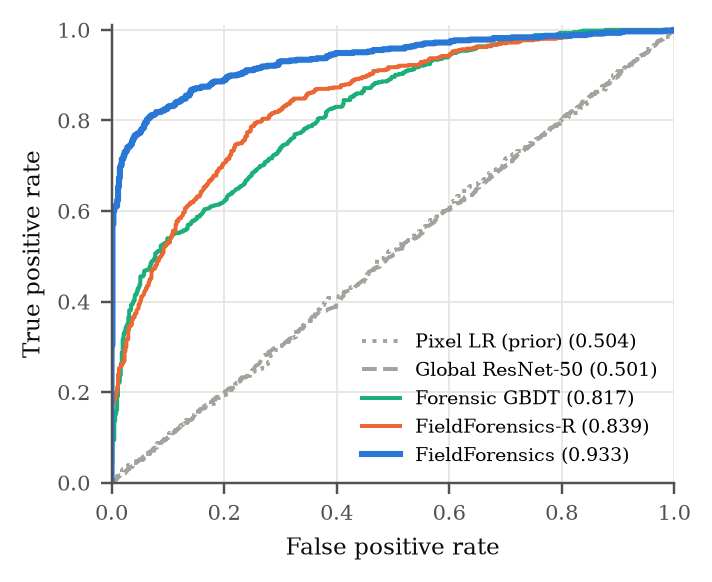
\includegraphics[width=\columnwidth]{figures/roc.png}
\caption{ROC curves on the paired test set (AUC in parentheses). FieldForensics-R is the degradation-augmented configuration.}
\label{fig:roc}
\end{figure}
Fig.~\ref{fig:scores} shows why the AUCs differ so much. The prior pixel baseline gives every page almost the same score. The forensic GBDT and FieldForensics-R produce broad, overlapping distributions. FieldForensics is nearly binary: most authentic pages score below 0.2, and most forgeries score close to 1.

\begin{figure*}[t]
\centering
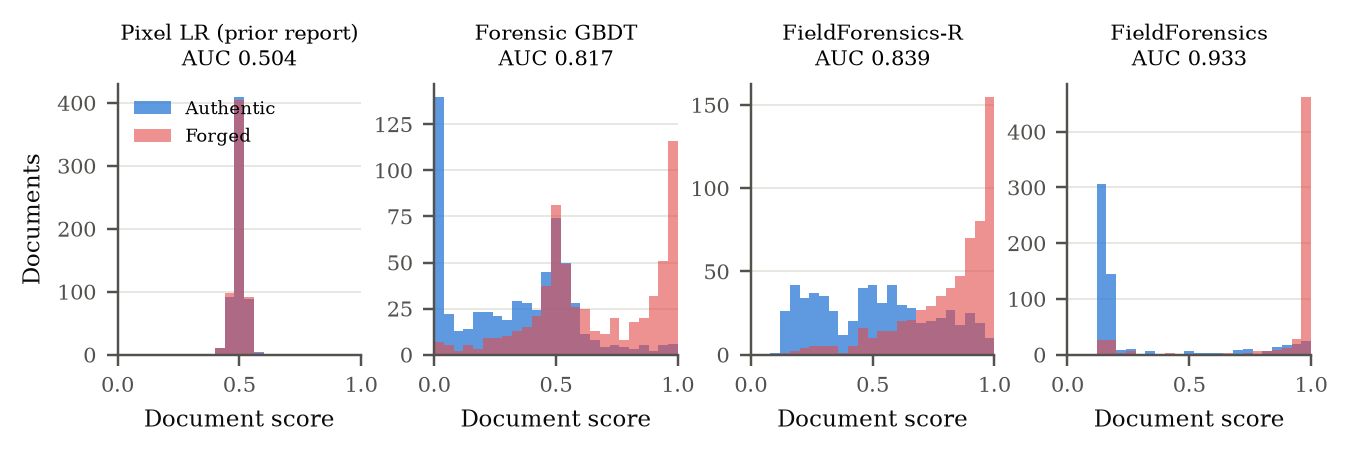
\includegraphics[width=\textwidth]{figures/score_dist.png}
\caption{Distribution of document scores for authentic (blue) and forged (red) test pages. From left to right the classes separate more cleanly, ending with FieldForensics, which assigns near-binary scores.}
\label{fig:scores}
\end{figure*}
\subsection{Per-source analysis and complementary cues}
\begin{table*}[t]
\centering
\caption{Per-source results (test split; storage format of the source release in parentheses). AUC of FieldForensics (FF, with 95\% CI), FieldForensics-R (FF-R), the forensic-statistics GBDT and the FF-R + GBDT fusion; paired accuracy, pixel F1 and peak-hit rate of FF}
\label{tab:source}
\footnotesize
\setlength{\tabcolsep}{3pt}
\begin{tabular}{lccccccc}
\toprule
Source & FF AUC [95\% CI] & FF-R & GBDT & FF-R + GBDT & Paired (\%) & Pix. F1 & Peak hit (\%) \\
\midrule
CORD (PNG) & 0.988 [0.977, 0.997] & 0.957 & 0.781 & 0.963 & 98.2 & 0.839 & 98.0 \\
WildReceipt (JPEG) & 0.902 [0.877, 0.926] & 0.810 & 0.856 & 0.890 & 87.6 & 0.600 & 83.5 \\
SROIE (JPEG) & 0.996 [0.988, 1.000] & 0.850 & 0.861 & 0.914 & 100.0 & 0.837 & 100.0 \\
XFUND (PNG) & 0.852 [0.802, 0.903] & 0.582 & 0.666 & 0.683 & 92.2 & 0.350 & 85.5 \\
\bottomrule
\end{tabular}
\end{table*}
Table~\ref{tab:source} breaks the results down by source. FieldForensics is strong on all four: CORD 0.988, WildReceipt 0.902, SROIE 0.996 and XFUND 0.852. The peak-hit rate reaches 100.0\% on the best source. XFUND forms remain the hardest case: their 2480$\times$3508 pages hold many crisp printed lines that can produce false peaks, and they make up only 14\% of the training documents. The comparison between FieldForensics-R and the forensic GBDT is revealing. On CORD, FieldForensics-R is far ahead (0.957 vs. 0.781). On the JPEG-distributed WildReceipt and SROIE receipts the hand-crafted statistics are better (0.856 vs. 0.810 and 0.861 vs. 0.850), and FieldForensics-R collapses on XFUND (0.582). A field regenerated by GPT-Image-2 and pasted into a page that was JPEG-compressed before the edit lacks the page's 8$\times$8 block-compression history, and ELA and blockiness statistics are designed to detect exactly this inconsistency \cite{catnet,doctamper}. Grouped permutation importance confirms what the GBDT relies on: shuffling the ELA features across test images lowers its AUC by 0.312, against 0.079 for the noise-residual features and 0.045 for blockiness. ELA measures how a region responds to one more JPEG compression, so it is a direct probe of compression history. Its importance even on CORD (0.275) suggests that the PNG-distributed CORD photographs also carry an earlier, camera-side JPEG history. The augmentation of FieldForensics-R re-compresses half of its training crops and so teaches the network to \emph{ignore} compression history. The fused FieldForensics-R + GBDT re-introduces that cue and is better than either component on every source. FieldForensics, trained without augmentation, learns both cues by itself: it beats the fusion on 4 of 4 sources, and adding the GBDT to it brings nothing. Score levels still differ between document types (the median score of authentic pages is 0.904 on XFUND but 0.151 on CORD), which is why the TPR at 5\% FPR (77.2\%) is lower than the paired accuracy suggests: a single global threshold is imperfectly calibrated across document types.

\begin{figure}[t]
\centering
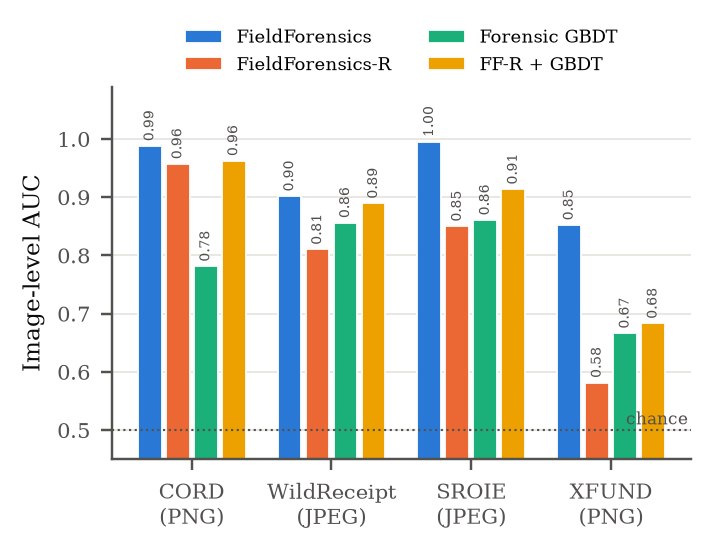
\includegraphics[width=\columnwidth]{figures/per_source.png}
\caption{Per-source AUC of the four strongest systems (values above bars). FieldForensics leads on every source; the hand-crafted compression statistics (GBDT) are competitive only on the JPEG-distributed receipts.}
\label{fig:persrc}
\end{figure}
Fig.~\ref{fig:size} groups the test documents into quartiles of forged area relative to the page (the smallest quartile covers 0.30\% of the page or less). The AUC is 0.922, 0.957, 0.907 and 0.966 from the smallest to the largest quartile. The smallest quartile is dominated by XFUND (83 of its 152 forged documents), because a form field is a tiny fraction of a large page. Excluding XFUND, the smallest quartile reaches 0.960 (dotted line), so any apparent effect of the relative edit size is largely a document-type effect. Pixel F1 increases with field size (from 0.555 to 0.755), as expected for a localisation metric dominated by boundary errors.

\begin{figure}[t]
\centering
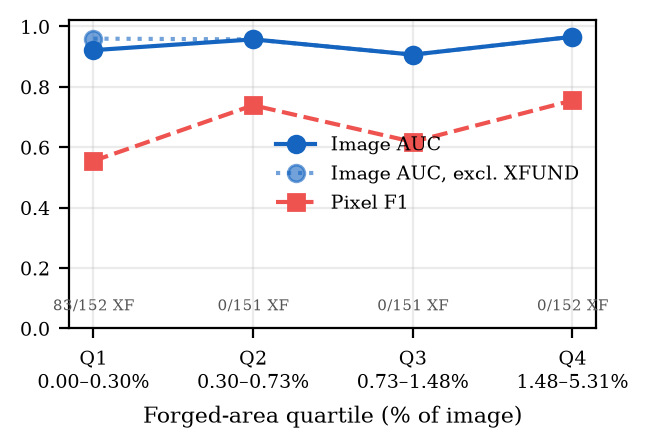
\includegraphics[width=\columnwidth]{figures/size.png}
\caption{Detection AUC and pixel F1 of FieldForensics against the forged area (quartiles of the percentage of page pixels that were regenerated). Labels give the number of XFUND documents per quartile.}
\label{fig:size}
\end{figure}
\subsection{Ablation study}
\begin{table}[t]
\centering
\caption{Ablations of FieldForensics-R (same training budget; ΔAUC relative to the full augmented model; $p$ from a paired bootstrap over test documents)}
\label{tab:abl}
\footnotesize
\setlength{\tabcolsep}{3pt}
\begin{tabular}{lcccccc}
\toprule
Variant & AUC & ΔAUC & $p$ & Paired (\%) & Pix. F1 & TPR@5\% \\
\midrule
FieldForensics-R (full) & 0.839 & -- & -- & 87.9 & 0.486 & 39.6 \\
-- SRM noise stream (RGB only) & 0.768 & -0.071 & <0.001 & 85.4 & 0.399 & 25.7 \\
-- paired hard negatives (uniform auth. crops) & 0.817 & -0.021 & <0.001 & 86.4 & 0.457 & 35.6 \\
-- pixel supervision (image labels only) & 0.500 & -0.339 & <0.001 & 52.7 & 0.000 & 5.0 \\
-- degradation augmentation (= FieldForensics) & 0.933 & +0.094 & <0.001 & 92.9 & 0.667 & 77.2 \\
\bottomrule
\end{tabular}
\end{table}
The ablations were run on the augmented configuration, which was our initial default (Table~\ref{tab:abl}). \emph{Noise stream.} Removing the SRM residual input changes the AUC from 0.839 to 0.768 (paired bootstrap $p<0.001$). High-pass residuals expose the generated glyphs' missing scan noise more directly than RGB alone. \emph{Paired hard negatives.} Sampling authentic crops uniformly instead of at the field location changes the AUC from 0.839 to 0.817 (paired bootstrap $p<0.001$) and lowers paired accuracy to 86.4\% and pixel F1 to 0.457. A plausible explanation is that, without paired negatives, the network can partly rely on the content shortcut ``numeric fields are suspicious'', which also fires on authentic documents \cite{geirhos}. \emph{Pixel supervision.} With image labels only, the top-$k$ pooled network does not learn at all within the budget (AUC 0.500, pixel F1 0.000). Finding a field that covers less than 1\% of the page from a single bit per image is a hard multiple-instance problem \cite{mil}, and the masks shipped with the benchmark are what make the task learnable at this scale. \emph{Degradation augmentation.} Removing the augmentation is the largest single change: the AUC rises from 0.839 to 0.933 (paired bootstrap $p<0.001$). The resulting model is FieldForensics; its cost in robustness is analysed next.

\emph{Pooling rule.} Turning the FieldForensics map into a document score by its raw maximum gives AUC 0.932, the smoothed maximum of Eq.~(\ref{eq:score}) 0.933, the mean of the top-256 pixels 0.930, and the global mean only 0.269. Peak-based pooling is essential: averaging dilutes a sub-1\% region with genuine pixels, which is the same failure mode as whole-page classification.

\subsection{Robustness to post-processing}
\begin{figure*}[t]
\centering
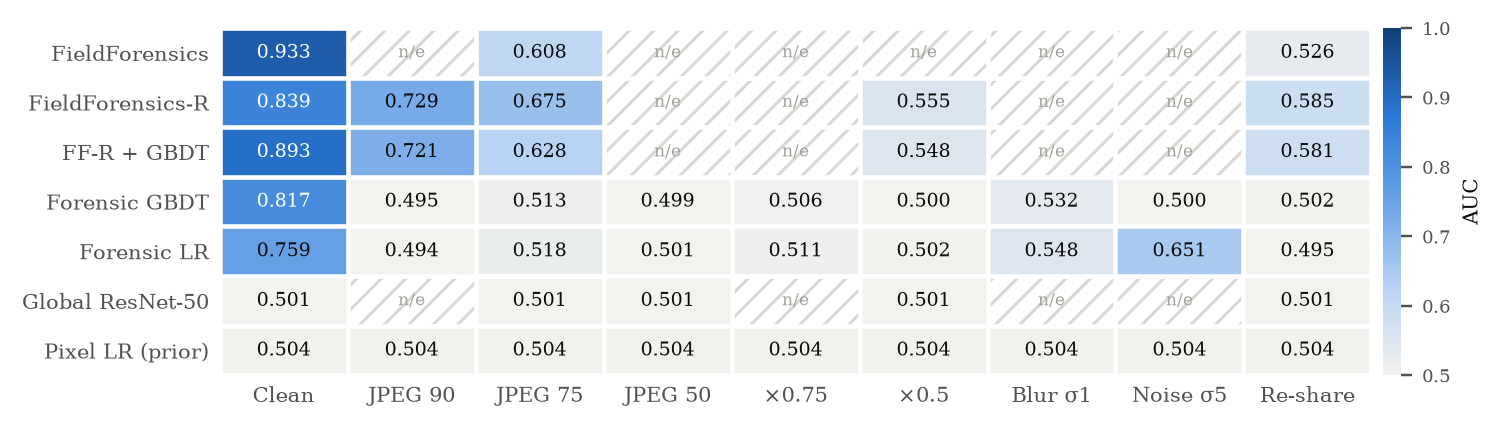
\includegraphics[width=\textwidth]{figures/robustness.png}
\caption{Image-level AUC under test-time degradations applied to the whole page (both classes alike): JPEG re-compression at quality 90/75/50, down-scaling to 75\%/50\%, Gaussian blur ($\sigma=1$), Gaussian noise ($\sigma=5$), and a messaging-app style re-share (75\% scale + JPEG 80). Darker cells mean higher AUC; hatched cells (n/e) were not evaluated because of the compute budget.}
\label{fig:robust}
\end{figure*}
Fig.~\ref{fig:robust} reports AUC under degradations applied to the whole page, so authentic and forged images are processed identically. FieldForensics drops from 0.933 on clean pages to 0.608 under JPEG quality 75 and 0.526 under the messaging-app re-share (75\% scale + JPEG 80). FieldForensics-R starts lower (0.839) and obtains 0.729 under JPEG quality 90, 0.675 under JPEG quality 75, 0.555 under down-scaling to 50\% and 0.585 under the messaging-app re-share (75\% scale + JPEG 80). Degradation augmentation therefore buys robustness at the price of clean accuracy: FieldForensics-R is ahead under JPEG quality 75 and the messaging-app re-share (75\% scale + JPEG 80), whereas FieldForensics is far ahead on pristine files. Which configuration to deploy depends on the channel through which documents arrive: original uploads favour FieldForensics, re-shared or re-compressed images favour FieldForensics-R, and a re-compression detector could select between them. The hand-crafted compression statistics are the most fragile: the forensic GBDT falls from 0.817 to 0.495 under JPEG quality 90, 0.513 under JPEG quality 75, 0.499 under JPEG quality 50, 0.506 under down-scaling to 75\%, 0.500 under down-scaling to 50\%, 0.532 under Gaussian blur, 0.500 under additive noise and 0.502 under the messaging-app re-share (75\% scale + JPEG 80), i.e. to chance. Their clean-data strength comes from the compression-history inconsistency of the pasted patch, which any re-compression, rescaling or blurring of the page erases. For the same reason the FieldForensics-R + GBDT fusion obtains 0.721 under JPEG quality 90, 0.628 under JPEG quality 75, 0.548 under down-scaling to 50\% and 0.581 under the messaging-app re-share (75\% scale + JPEG 80), below FieldForensics-R alone, so a compression branch must be gated by a re-compression check before it is trusted. Per source (Fig.~\ref{fig:robsrc}), JPEG 75 costs FieldForensics 0.27--0.36 AUC on every source (CORD 0.362, WildReceipt 0.279, SROIE 0.271, XFUND 0.303), including the PNG-distributed ones. This is consistent with a network whose fine-grained evidence, both generator traces and compression history, is largely overwritten by one more round of compression. The global ResNet-50 is at chance under every condition.

\begin{figure}[t]
\centering
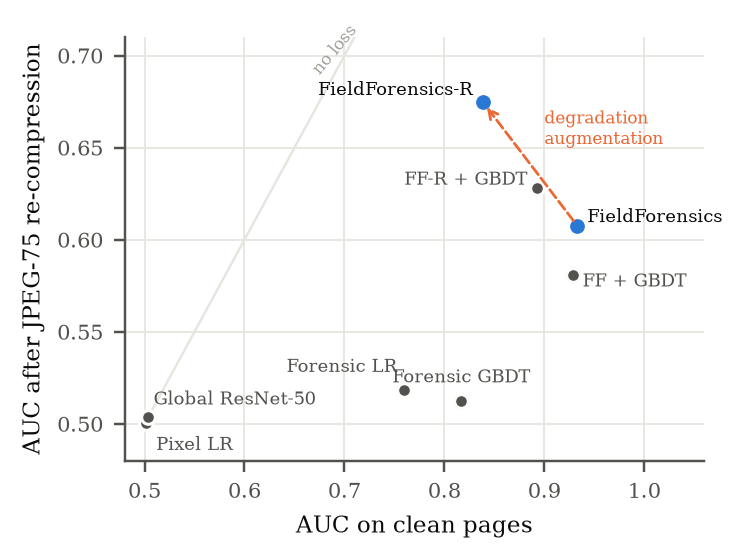
\includegraphics[width=\columnwidth]{figures/tradeoff.png}
\caption{The accuracy--robustness trade-off: clean AUC against AUC after JPEG-75 re-compression of the page. Degradation augmentation (arrow) moves the network from the most accurate to the most robust operating point; the grey diagonal would mean no loss at all.}
\label{fig:tradeoff}
\end{figure}
Fig.~\ref{fig:tradeoff} summarises this trade-off. No system lies close to the diagonal. Every detector loses evidence under re-compression, and choosing between FieldForensics and FieldForensics-R means choosing a point on this frontier.

\begin{figure}[t]
\centering
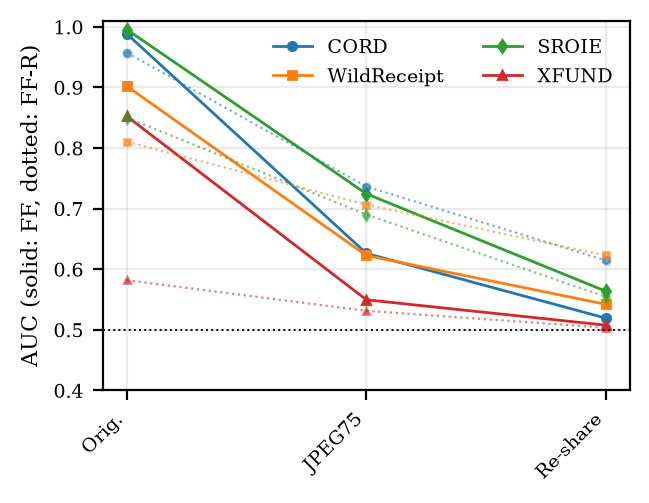
\includegraphics[width=\columnwidth]{figures/robust_source.png}
\caption{Per-source AUC under degradations for FieldForensics (solid) and FieldForensics-R (dotted). WildReceipt and SROIE are distributed as JPEG files, CORD and XFUND as PNG.}
\label{fig:robsrc}
\end{figure}
\subsection{Generalisation to an unseen document source}
\begin{table}[t]
\centering
\caption{Leave-one-source-out (FieldForensics-R configuration): test documents of a source scored by the model trained on all sources (in) and by a model trained without that source (out)}
\label{tab:loso}
\footnotesize
\setlength{\tabcolsep}{3pt}
\begin{tabular}{lcccccc}
\toprule
Held-out & AUC in & AUC out [95\% CI] & Pair in & Pair out & F1 in & F1 out \\
\midrule
CORD & 0.957 & 0.745 [0.715, 0.777] & 99.5 & 87.2 & 0.642 & 0.354 \\
\bottomrule
\end{tabular}
\end{table}
To probe generalisation, we retrain the network (augmented configuration) with one source removed from training and validation and test it on that source's test documents (Table~\ref{tab:loso}). CORD goes from 0.957 in-domain to 0.745 when held out. Generator traces learned on one document population thus transfer only partially, and diverse training sources matter.

\subsection{Qualitative results}
\begin{figure*}[t]
\centering
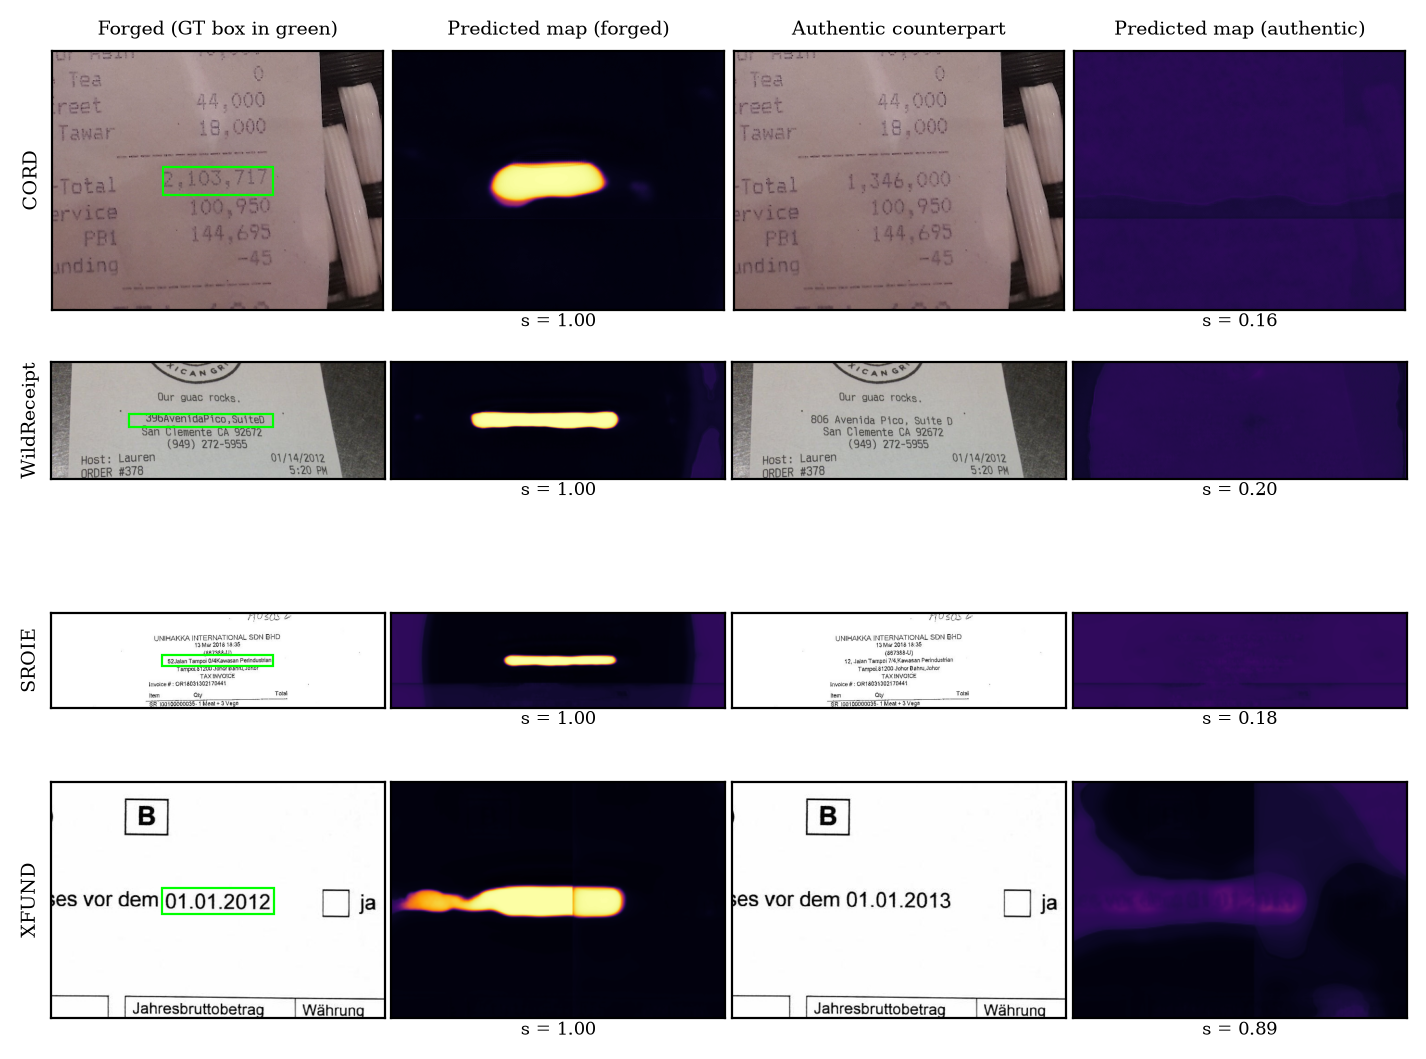
\includegraphics[width=\textwidth]{figures/qualitative.png}
\caption{FieldForensics tampering maps for one test document per source (context window around the field). For each document the forged version (left pair) and its authentic counterpart (right pair) are shown with the document score $s$. The network is evaluated on full pages; crops are for display only.}
\label{fig:qual}
\end{figure*}
Fig.~\ref{fig:qual} illustrates typical behaviour. On forged pages the edited value produces a compact, high-confidence blob, while the authentic counterpart yields a flat, low map. The maps are blob-shaped rather than following individual strokes, which limits pixel F1 even when the field is found. On large XFUND forms the authentic page can also produce elevated responses along printed lines, which is the main source of false alarms. Because the network outputs a localisation, an analyst can check every alarm by inspecting the highlighted field instead of trusting an opaque page-level score.

\section{Discussion}\label{sec:disc}
\emph{Why whole-page classification fails.} With a median forged area of 0.76\%, an authentic page and its forgery share more than 99\% of their pixels, and in the paired protocol they share everything else as well: layout, source, language and resolution. A page-level descriptor that pools uniformly over the image, such as a resized CNN input or a pixel histogram, averages the evidence away. Every method that works here, FieldForensics as well as the block-wise forensic statistics, keeps the evidence local and at native resolution and pools by maxima. Paired hard negatives keep the network from substituting content priors for forensic evidence. We think this \emph{localize-to-detect} view is the right default for any local generative edit, not only for receipts.

\emph{What is being detected.} Two families of cues are available. The first is the generator's own signature: the decoding and up-sampling structure of the image model, which renders glyphs whose noise and stroke texture differ from scanned or photographed ink. The second is an \emph{interface} cue: the pasted patch has a different compression history, sharpness and noise level from the page around it. Our experiments separate the two. Block-wise compression statistics see only interface cues: they are competitive on JPEG-distributed receipts but fall to chance after any re-compression. FieldForensics-R, whose augmentation suppresses compression cues, is weaker on clean data and needs the GBDT to recover them. The clean-trained FieldForensics learns both families and gains nothing from the GBDT. Interface cues are strong but fragile, and a careful forger could suppress them by re-saving the whole page. A deployable system should therefore treat re-compression as a first-class condition, as we do here, and combine pixel evidence with non-pixel checks such as arithmetic consistency of totals, issuer databases and provenance metadata (e.g., C2PA).

\emph{Relation to the published zero-shot results.} TruFor and DocTamper were not trained on generative field edits, and their low AUCs \cite{aiforge2} measure transfer, not the learnability of the task. Our results show that the task \emph{is} learnable from about two thousand paired examples on a single consumer GPU. The flip side is that a supervised detector inherits the biases of its training generator, sources and file-handling pipeline. Generalisation to other generators (e.g., the Gemini and Ideogram forgeries of AIForge-Doc v1) remains the critical open question.

\emph{Ethical considerations.} The dataset contains real receipts and forms released for research under non-commercial licences, and our models detect forgeries rather than create them. Reporting where detectors fail could inform forgers, but the failure modes we identify (re-compression, large-format pages) are already common knowledge in image forensics, and making them explicit helps practitioners avoid over-trusting automated checks. A detector score should support, not replace, human review and procedural controls.

\section{Limitations and Future Work}\label{sec:lim}
\begin{itemize}
\item \textbf{Fragility to re-sharing.} Both configurations lose much of their accuracy when the page is re-compressed or rescaled. The best clean detector is not the most robust one, and closing this gap, for example with longer training or curriculum augmentation, is the most pressing practical problem.
\item \textbf{Single generator.} All forgeries come from GPT-Image-2, so the detector may be specific to its artefacts. Cross-generator evaluation on AIForge-Doc v1 (Gemini 2.5 Flash Image, Ideogram v2) is the most important next step.
\item \textbf{Compute budget.} All networks were trained for a short, equal budget (1,500 iterations, about 35 minutes) on a 6\,GB laptop GPU that was thermally throttled during the experiments, and each variant was run with a single seed. Bootstrap intervals capture test-sample uncertainty but not training variance.
\item \textbf{Large-format forms and calibration.} XFUND remains the hardest source, and score levels differ between document types, so per-type thresholds are needed in practice.
\item \textbf{Simulated degradations and paste-back forgeries.} Degradations were simulated digitally; print--scan and camera re-capture are not covered. The benchmark pastes the regenerated field back into the original page, whereas a forger who regenerates or re-photographs the whole page would remove the interface cues.
\item \textbf{Benchmark scale.} 606 test documents give AUC intervals of roughly $\pm$0.01--0.03 overall and wider ones per source (SROIE has 60 test documents).
\end{itemize}
Future work will train on mixtures of generators, add a JPEG-DCT stream as in CAT-Net \cite{catnet}, use OCR to restrict attention to text lines, combine pixel evidence with semantic checks (e.g., totals that do not add up), and test on physically printed and re-captured documents.

\section{Conclusion}\label{sec:concl}
We revisited the detection of AI-generated field forgeries in receipts and forms on the AIForge-Doc v2 benchmark. After de-duplicating the data and adopting a strictly paired protocol, we showed that classifying down-sampled whole pages fails because the edit is too small, and that evidence must be gathered locally and at native resolution. FieldForensics localises tampering with an RGB--noise U-Net trained on field-centred crops with paired hard negatives, and scores a page by the peak of its map. It reaches an AUC of 0.933, a paired 2AFC accuracy of 92.9\% and a pixel F1 of 0.667, where humans and published zero-shot detectors are at 0.50--0.60, and it points to the forged field. Our analysis shows that such a detector exploits both generator traces and compression-history inconsistencies. The latter make block-wise forensic statistics a strong baseline on pristine files, but they vanish under re-compression. Training for robustness to degradations trades clean accuracy for robustness, and re-shared documents remain the main open problem. Our splits, code and per-image predictions will be made available to support further work on this threat.

\section*{Acknowledgment}
The author thanks the creators of AIForge-Doc and of the CORD, WildReceipt, SROIE and XFUND corpora for releasing their data for research use.

\begin{thebibliography}{99}
\bibitem{findit} C. Artaud, N. Sid\`ere, A. Doucet, J.-M. Ogier, and V. Poulain D'Andecy, ``Find it! Fraud detection contest report,'' in \emph{Proc. 24th Int. Conf. Pattern Recognit. (ICPR)}, 2018, pp. 13--18.
\bibitem{doctamper} C. Qu, C. Liu, Y. Liu, X. Chen, D. Peng, F. Guo, and L. Jin, ``Towards robust tampered text detection in document image: New dataset and new solution,'' in \emph{Proc. IEEE/CVF CVPR}, 2023, pp. 5937--5946.
\bibitem{catnet} M.-J. Kwon, S.-H. Nam, I.-J. Yu, H.-K. Lee, and C. Kim, ``Learning JPEG compression artifacts for image manipulation detection and localization,'' \emph{Int. J. Comput. Vis.}, vol. 130, pp. 1875--1895, 2022.
\bibitem{aiforge1} J. Wu, Y. Zhou, M. Xu, Z. Liang, S. Ren, J. Xue, M. Yang, S. Chen, and J. Huan, ``AIForge-Doc: A benchmark for detecting AI-forged tampering in financial and form documents,'' arXiv:2602.20569, 2026.
\bibitem{aiforge2} J. Wu, Y. Zhou, D. Tsang Ng, X. Shen, K. Zewde, A. Raj, T. Duong, and S. Ren, ``AIForge-Doc v2: A paired benchmark of GPT-Image-2 document forgeries,'' dataset, Hugging Face (Scam-AI/AIForge-Doc-v2), 2026.
\bibitem{cord} S. Park, S. Shin, B. Lee, J. Lee, J. Surh, M. Seo, and H. Lee, ``CORD: A consolidated receipt dataset for post-OCR parsing,'' in \emph{NeurIPS Workshop on Document Intelligence}, 2019.
\bibitem{wildreceipt} H. Sun, Z. Kuang, X. Yue, C. Lin, and W. Zhang, ``Spatial dual-modality graph reasoning for key information extraction,'' arXiv:2103.14470, 2021.
\bibitem{sroie} Z. Huang, K. Chen, J. He, X. Bai, D. Karatzas, S. Lu, and C. V. Jawahar, ``ICDAR2019 competition on scanned receipt OCR and information extraction,'' in \emph{Proc. ICDAR}, 2019, pp. 1516--1520.
\bibitem{xfund} Y. Xu, T. Lv, L. Cui, G. Wang, Y. Lu, D. Florencio, C. Zhang, and F. Wei, ``XFUND: A benchmark dataset for multilingual visually rich form understanding,'' in \emph{Findings of ACL}, 2022, pp. 3214--3224.
\bibitem{trufor} F. Guillaro, D. Cozzolino, A. Sud, N. Dufour, and L. Verdoliva, ``TruFor: Leveraging all-round clues for trustworthy image forgery detection and localization,'' in \emph{Proc. IEEE/CVF CVPR}, 2023, pp. 20606--20615.
\bibitem{forgerjudge} J. Wu, Y. Zhou, D. Tsang Ng \emph{et al.}, ``When the forger is the judge: GPT-Image-2 cannot recognize its own faked documents,'' arXiv:2604.25213, 2026.
\bibitem{unet} O. Ronneberger, P. Fischer, and T. Brox, ``U-Net: Convolutional networks for biomedical image segmentation,'' in \emph{Proc. MICCAI}, 2015, pp. 234--241.
\bibitem{resnet} K. He, X. Zhang, S. Ren, and J. Sun, ``Deep residual learning for image recognition,'' in \emph{Proc. IEEE/CVF CVPR}, 2016, pp. 770--778.
\bibitem{srm} J. Fridrich and J. Kodovsk\'y, ``Rich models for steganalysis of digital images,'' \emph{IEEE Trans. Inf. Forensics Security}, vol. 7, no. 3, pp. 868--882, 2012.
\bibitem{rgbn} P. Zhou, X. Han, V. I. Morariu, and L. S. Davis, ``Learning rich features for image manipulation detection,'' in \emph{Proc. IEEE/CVF CVPR}, 2018, pp. 1053--1061.
\bibitem{mantra} Y. Wu, W. AbdAlmageed, and P. Natarajan, ``ManTra-Net: Manipulation tracing network for detection and localization of image forgeries with anomalous features,'' in \emph{Proc. IEEE/CVF CVPR}, 2019, pp. 9543--9552.
\bibitem{mvss} X. Chen, C. Dong, J. Ji, J. Cao, and X. Li, ``Image manipulation detection by multi-view multi-scale supervision,'' in \emph{Proc. IEEE/CVF ICCV}, 2021, pp. 14185--14193.
\bibitem{wang2020} S.-Y. Wang, O. Wang, R. Zhang, A. Owens, and A. A. Efros, ``CNN-generated images are surprisingly easy to spot... for now,'' in \emph{Proc. IEEE/CVF CVPR}, 2020, pp. 8695--8704.
\bibitem{corvi} R. Corvi, D. Cozzolino, G. Zingarini, G. Poggi, K. Nagano, and L. Verdoliva, ``On the detection of synthetic images generated by diffusion models,'' in \emph{Proc. IEEE ICASSP}, 2023.
\bibitem{ojha} U. Ojha, Y. Li, and Y. J. Lee, ``Towards universal fake image detectors that generalize across generative models,'' in \emph{Proc. IEEE/CVF CVPR}, 2023, pp. 24480--24489.
\bibitem{li2025} Z. Li, J. Yan, Z. He, K. Zeng, W. Jiang, L. Xiong, and Z. Fu, ``Is artificial intelligence generated image detection a solved problem?'' in \emph{Advances in Neural Information Processing Systems (NeurIPS)}, 2025.
\bibitem{hpfcn} H. Li and J. Huang, ``Localization of deep inpainting using high-pass fully convolutional network,'' in \emph{Proc. IEEE/CVF ICCV}, 2019, pp. 8301--8310.
\bibitem{fu2026} Z. Fu, J. Yan, Y. Chen, X. Yu, Y. Li, H. Jiang, L. Gao, and C. Bao, ``Beyond natural images: Rethinking AI-generated image detection in documents,'' arXiv:2609.14352, 2026.
\bibitem{bootstrap} B. Efron and R. J. Tibshirani, \emph{An Introduction to the Bootstrap}. New York, NY, USA: Chapman \& Hall, 1993.
\bibitem{mil} M. Ilse, J. M. Tomczak, and M. Welling, ``Attention-based deep multiple instance learning,'' in \emph{Proc. ICML}, 2018, pp. 2127--2136.
\bibitem{imagenet} J. Deng, W. Dong, R. Socher, L.-J. Li, K. Li, and L. Fei-Fei, ``ImageNet: A large-scale hierarchical image database,'' in \emph{Proc. IEEE/CVF CVPR}, 2009, pp. 248--255.
\bibitem{geirhos} R. Geirhos, J.-H. Jacobsen, C. Michaelis, R. Zemel, W. Brendel, M. Bethge, and F. A. Wichmann, ``Shortcut learning in deep neural networks,'' \emph{Nature Mach. Intell.}, vol. 2, pp. 665--673, 2020.
\bibitem{vnet} F. Milletari, N. Navab, and S.-A. Ahmadi, ``V-Net: Fully convolutional neural networks for volumetric medical image segmentation,'' in \emph{Proc. 3DV}, 2016, pp. 565--571.
\bibitem{ela} N. Krawetz, ``A picture's worth: Digital image analysis and forensics,'' in \emph{Black Hat Briefings USA}, 2007.
\bibitem{sklearn} F. Pedregosa \emph{et al.}, ``Scikit-learn: Machine learning in Python,'' \emph{J. Mach. Learn. Res.}, vol. 12, pp. 2825--2830, 2011.
\bibitem{pytorch} A. Paszke \emph{et al.}, ``PyTorch: An imperative style, high-performance deep learning library,'' in \emph{Advances in Neural Information Processing Systems (NeurIPS)}, 2019, pp. 8024--8035.
\bibitem{adamw} I. Loshchilov and F. Hutter, ``Decoupled weight decay regularization,'' in \emph{Proc. ICLR}, 2019.
\end{thebibliography}
\end{document}